\documentclass[12pt]{article}

% Style
\usepackage{parskip}	% Blank line between paragraphs
\usepackage[top=1in, bottom=1.25in, left=1.25in, right=1.25in]{geometry} % Page margins
\usepackage{float} % Placement of figures with H
\renewcommand{\familydefault}{\sfdefault} % Use sans-serif font (https://tex.stackexchange.com/a/2097)

% Maths
\usepackage{graphicx}
\usepackage{amsmath}
\usepackage{amssymb}
\usepackage{units}

\usepackage[hidelinks, pdfusetitle]{hyperref}

% Utillities
\usepackage{framed} % Draw frames around paragraphs
\usepackage{listings} % Code listings
\usepackage{color}
\usepackage{array}

% Settings
\allowdisplaybreaks		% Break aligned equations over pages

\usepackage{perpage}      % Reset footnote counter per page (1)
\MakePerPage{footnote}    % Reset footnote counter per page (2)

% Change itemize label items
\renewcommand{\labelitemi}{$\bullet$}
\renewcommand{\labelitemii}{$\bullet$}
\renewcommand{\labelitemiii}{$\bullet$}

% Parameters
\newcommand{\version}{0.6.1}
\newcommand{\website}{\href{http://www.virtualbow.org/}{\texttt{\textcolor{blue}{http://www.virtualbow.org/}}}}
\newcommand{\copyrights}{Copyright (C) 2016-2018 Stefan Pfeifer}

\begin{document}

\begin{titlepage}

\vspace*{5em}
\centering{\Huge\textbf{VirtualBow~v\version \\[1em] User Manual}}

\vspace{5em}

\centerline{
\includegraphics[width=0.2\textwidth]{figures/logo.png}}

\null
\vfill
\centerline{\copyrights}

\thispagestyle{empty}
\end{titlepage}

\newpage
\tableofcontents

\newpage
\section{Introduction}
\bigskip

This is the user manual for VirtualBow, a software tool for bow and arrow physics simulation.
It shows how to use the program, explains the various input parameters and results and also contains some additional background information.

For the latest version of the software and this manual visit the project's website at\\
\website.\\

\newpage
\section{The Bow Editor}

The bow editor is the main window of the application. Here you can load, edit and save bow models and start static and dynamic simulations.

\begin{figure}[H]
\centering
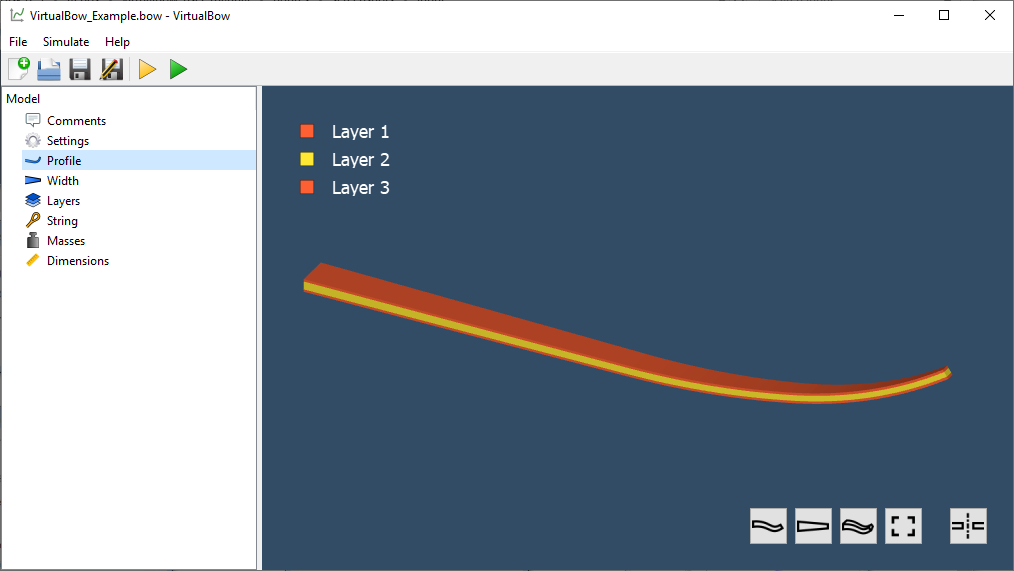
\includegraphics[width=\textwidth]{figures/screenshots/input/bow-editor}
\caption{Bow Editor}
\label{fig:bow-editor}
\end{figure}

Double-click any of the items on the left to edit the respective model properties. The 3D view on the right shows the current limb geometry.
Use the mouse to rotate (left mouse button), shift (middle mouse button) and zoom the view.
More view options are available through the buttons on the bottom-right corner.

\newpage
\subsection{Profile}

The profile curve is the geometric centerline of the bow limbs in unbraced state.
Use the table on the left to edit the parameters.
The result is shown on the plot on the right.

\begin{figure}[H]
\centering
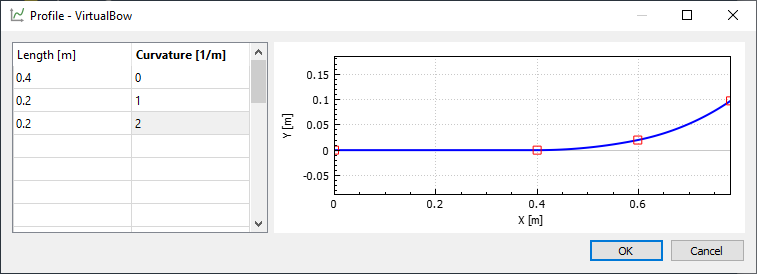
\includegraphics[width=\textwidth]{figures/screenshots/input/profile}
\caption{Profile dialog}
\label{fig:profile}
\end{figure}

The profile curve consists of a series of arc segments that each have a certain length and curvature. Each row in the table defines one such segment.

\textbf{Note:} Mathematically, the curvature $\kappa$ of a segment is the reciprocal of its radius $r$, so you can calculate the curvature via $\kappa = \frac{1}{r}$ if you know the radius and vice versa.

\newpage
\subsection{Width}

The width dialog is used to define the limb's width along its profile curve. This width is the same for all layers of the bow.

\begin{figure}[H]
\centering
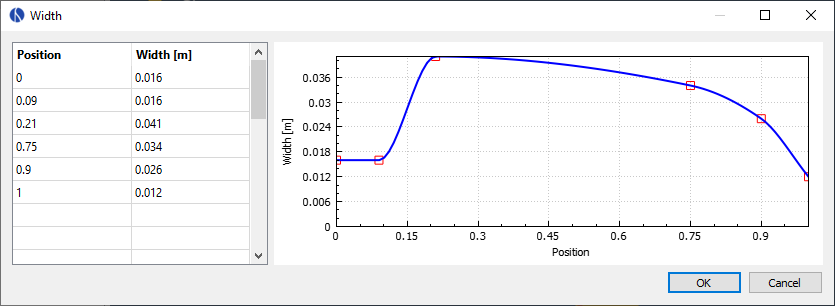
\includegraphics[width=\textwidth]{figures/screenshots/input/width}
\caption{Width dialog}
\label{fig:width}
\end{figure}

On the table on the left you can specify values for the width at certain relative positions (between 0 and 1) along the limb's profile curve. This definition of cross section properties relative to the total length of the profile curve makes it possible to change the profile without having to adjust any cross sections.

The actual width distribution of the limb is constructed as a smooth curve (monotonic cubic spline) passing through the supplied values as shown on the plot on the right.

\newpage
\subsection{Layers}

With the layer dialog you can create any number of layers and specify their height/thickness and material properties.

\begin{figure}[H]
\centering
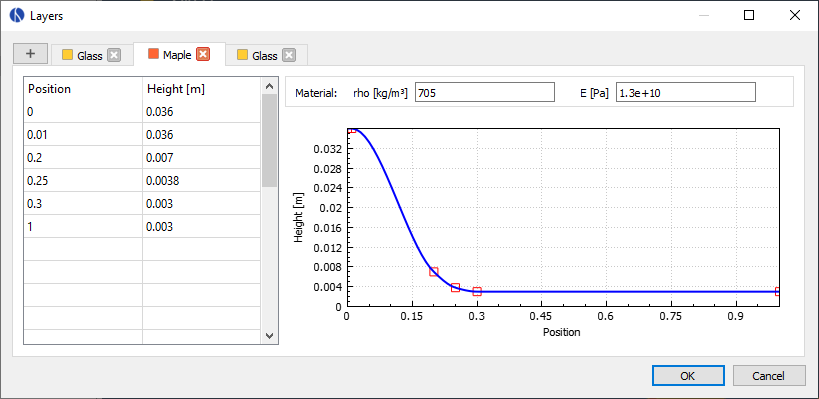
\includegraphics[width=\textwidth]{figures/screenshots/input/layers}
\caption{Layer dialog}
\label{fig:width}
\end{figure}

Click the plus button on the top left to add layers. You can later rearrange them by dragging the tabs. Double-click on a tab to rename a layer.

The table on the left sets the height distribution of the layer. It works the same way as the limb's width: You specify a number of values at different relative positions and the program creates an interpolating curve.

The layer material is specified by the following two constants,

\begin{itemize}
\item \textbf{rho:} Density (Mass per unit volume)
\item \textbf{E:} Elastic modulus (Measure for the stiffness of a solid material)
\end{itemize}

For manufactured materials like e.g. fiberglass or steel you might find those numbers in a datasheet provided by the manufacturer.

Wood is a bit more difficult, because the properties can vary quite a bit even within the same type.
You can find average numbers on the internet, for example at \url{http://www.wood-database.com}.
Those are probably good enough as a first reference.
However, in order to be really sure about a specific piece of wood there is no other way than to test it.
One possibility is a bending test as shown in Appendix~\ref{sec:bending-test}.

\newpage
\subsection{String}

Here you can define the mechanical properties of the string by providing data for the string material and the number of strands being used.

\begin{figure}[H]
\centering
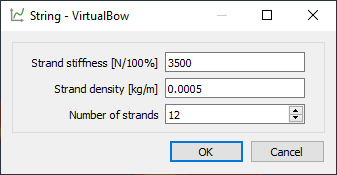
\includegraphics[width=0.4\textwidth]{figures/screenshots/input/string}
\caption{String dialog}
\label{fig:string}
\end{figure}

\begin{itemize}
\item \textbf{Strand density:} Linear density of the strands (mass per unit length)
\item \textbf{Strand stiffness:} Stiffness of the strands against elongation (force per unit strain)
\item \textbf{Number of strands:} Total number of strands in the string
\end{itemize}

The linear density of a string material can be easily determined with a kitchen scale (weight divided by length), but the stiffness is much more difficult to obtain.
Table~\ref{tbl:string-materials} shows some reference values taken from the SuperTiller V6.6 Excel spreadsheet by Alan Case\footnote{\url{http://www.buildyourownbow.com/build-alongs/how-to-use-supertiller-build-along/}}.

\textbf{Note:} The stiffness of the string material is an important parameter in dynamic analysis.
The static results however aren't affected very much by it as long as it is high enough to prevent significant elongation.

\begin{table}[H]
\centering
\begin{tabular}{ | p{60pt} | p{50pt} | p{50pt} | p{65pt} | p{140pt} | }
\hline
\textbf{Material}    & \textbf{Stiffness} [\unitfrac{N}{100\%}] & \textbf{Density} [\unitfrac{kg}{m}] & \textbf{Breaking strength} [\unit{N}] & \textbf{Source/Comment}\\ \hline
Dacron B50  & 3113.76  & 0.000333 & 217.96  & BCY assuming 7\% elongation at break (linearized)   \\ \hline
Fast Flight & 14086.04 & 0.000182 & 422.58  & BCY assuming 3\% elongation at break (linearized)   \\ \hline
Dyneema     & 18860.46 & 0.000160 & 578.27  & Calculated assuming linear stress-strain (to break) \\ \hline
Linen 40/3  & 1668.08  & 0.0642   & 49.38   & Maurice Taylor, Archery The Technical Side, 1947    \\ \hline
Silk        & 1026.51  & 0.0930   & 65.83   & Maurice Taylor, Archery The Technical Side, 1947    \\ \hline
\end{tabular}
\caption{Properties of common bowstring materials according to SuperTiller V6.6}
\label{tbl:string-materials}
\end{table}

\newpage
\subsection{Masses}

This dialog is usede to define the various masses of the bow. All of them except the arrow mass are optional.

\begin{figure}[H]
\centering
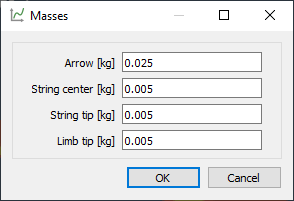
\includegraphics[width=0.4\textwidth]{figures/screenshots/input/masses}
\caption{Masses dialog}
\label{fig:masses}
\end{figure}

\begin{itemize}
\item \textbf{Arrow:} Mass of the arrow
\item \textbf{String center:} Additional mass at the string center (serving, nocking point)
\item \textbf{String tip:} Additional mass at the ends of the string (serving, silencers)
\item \textbf{Limb tip:} Additional mass at the limb tip (nocks, overlays)
\end{itemize}

\subsection{Dimensions}

The parameters listed in this dialog define the lengths and angles of the bow and its optional middle section/grip. See also figure~\ref{fig:dimensions-2} for a visual explanation of those parameters.


\begin{figure}[H]
\centering
\includegraphics[width=0.4\textwidth]{figures/screenshots/input/dimensions}
\caption{Dimensions dialog}
\label{fig:dimensions-1}
\end{figure}

\newpage
\begin{itemize}
\item{Draw}
\begin{itemize}
\item \textbf{Brace height:} Distance of the string center to the coordinate origin in braced state
\item \textbf{Draw length:} Distance of the string center to the coordinate origin in fully drawn state
\end{itemize}
\item{Handle}
\begin{itemize}
\item \textbf{Length:} Length of the riser or stiff middle section
\item \textbf{Setback:} Depth of the riser or stiff middle section
\item \textbf{Angle:} Angle of the riser or stiff middle section
\end{itemize}
\end{itemize}

\begin{figure}[H]
\centering
\includegraphics[width=0.4\textwidth]{figures/dimensions}
\caption{Dimensions of the bow}
\label{fig:dimensions-2}
\end{figure}

\newpage
\subsection{Comments}

The comments are meant for documenting the bow model. Any notes about the bow and the simulation results can be added here.

\begin{figure}[H]
\centering
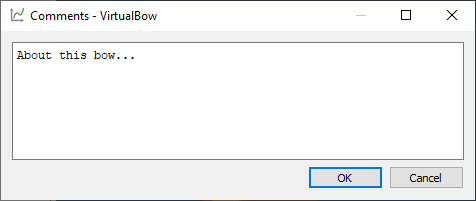
\includegraphics[width=0.7\textwidth]{figures/screenshots/input/comments}
\caption{Comments dialog}
\label{fig:comments}
\end{figure}

\subsection{Settings}

These are numerical settings that can be used to tweak the simulation.
Most of the time the default values should be fine though.
However, as the default values favor accuracy and realiability over performance there might be use cases where finding faster settings is worth it.
Think about running a large number of simulations with a script for example.

\begin{figure}[H]
\centering
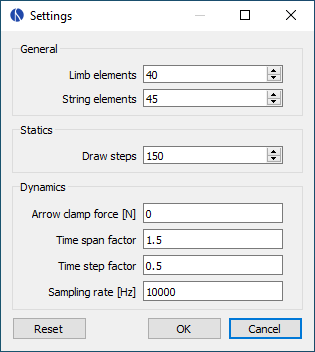
\includegraphics[width=0.4\textwidth]{figures/screenshots/input/settings}
\caption{Settings dialog}
\label{fig:settings}
\end{figure}

\newpage
These are the individual settings:

\begin{itemize}
\item \textbf{General}
    \begin{itemize}
    \item \textbf{Limb elements:} Number of finite elements that are used to approximate the limb. More elements increase the accuracy but also the computing time.
    \item \textbf{String elements:} Same as above.
    \end{itemize}
\item \textbf{Statics}
    \begin{itemize}
    \item \textbf{Draw steps:} Number of steps that are performed by the static simulation from brace height to full draw. This determines the resolution of the static results. You can usually decrease this value to speed up the simulation.
    \end{itemize}
\item \textbf{Dynamics}
    \begin{itemize}
    \item \textbf{Time span factor:} This controls the time period that is simulated. A value of $1$ corresponds to the time at which the arrow reaches brace height. The default value is larger than that in order to capture some of the things that occur after the arrow left the bow (maximum dynamic loads on limb and string).
    \item \textbf{Time step factor:} When carrying out the dynamic simulation the program will repeatedly use the current state of the bow at time $t$ to calculate the next state at time $t + \Delta t$ where $\Delta t$ is some small timestep. This timestep has to be chosen small enough to get an accurate and stable solution but also as large as possible to keep the number of steps low. The program can estimate this, but to be on the safe side the estimation is multiplied with a safety factor between $0$ and $1$ that you can choose here.
    \item \textbf{Sampling rate:} Limits the time resolution of the output data. This is done because the dynamic simulation usually produces much finer grained data than is actually useful. Not including all of that in the final output saves time and memory.
    \end{itemize}
\end{itemize}

\newpage
\section{Simulation Results}

You can start static or dynamic simulations by using the yellow and green toolbar buttons or the simulation menu.
A new window with the results will open once the simulation has finished.

\begin{figure}[H]
\centering
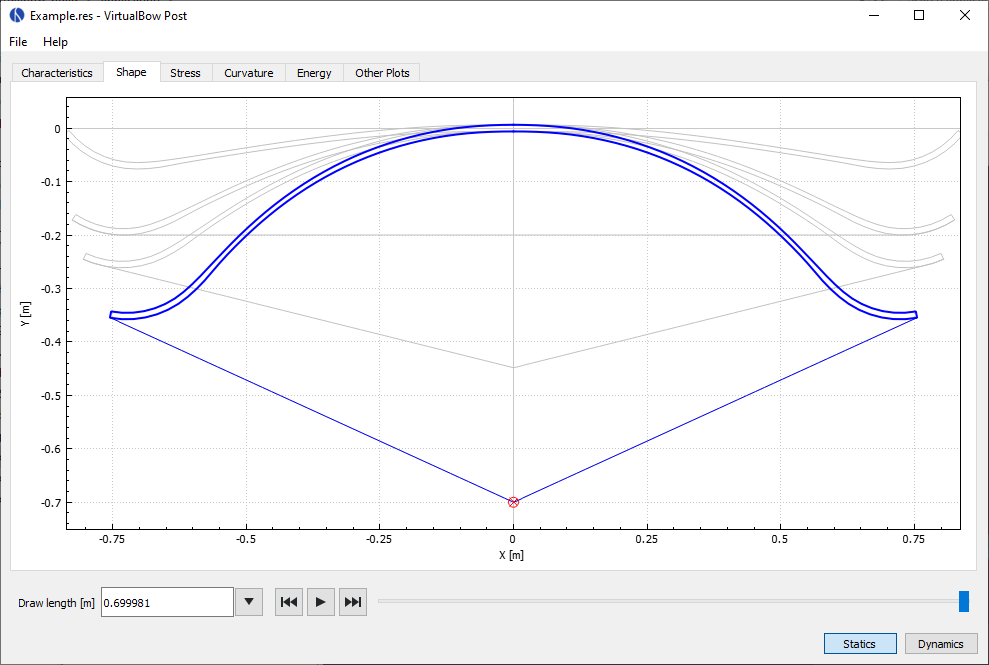
\includegraphics[width=\textwidth]{figures/screenshots/output/result-window}
\caption{Simulation results}
\label{fig:result-window}
\end{figure}

With the buttons on the bottom left you can switch between the static and dynamic (if available) results.
The results themselves are organized in different tabs.
At the bottom of the window there is a slider where you can change the current draw length (statics) or time (dynamics).
This value applies to all of the result tabs.

\newpage
These are the contents of the individual result tabs:

\begin{itemize}
\item \textbf{Shape:} Shows the shape of the limb and string as well as the position of the arrow at different stages of either the draw (statics) or the shot (dynamics)
\item \textbf{Stress:} Shows the distribution of material stress along the length of the limb for the back and belly of each layer
\item \textbf{Curvature:} Shows the curvature of the limb (difference to unbraced state)
\item \textbf{Energy:} Shows how potential and kinetic energy of the different parts of the bow develop during the simulation
\item \textbf{Other Plots:} Here you can combine arbitrary simulation results and plot them together, e.g. things like the draw curve of the bow or the velocity of the arrow.
\\
\item \textbf{Special Values (Statics):}
    \begin{itemize}
    \item \textbf{String length:} Initial length of the string such that the bow meets the specified brace height
    \item \textbf{Final draw force:} Draw force in fully drawn state
    \item \textbf{Drawing work:} Total work done by drawing the bow.
    \item \textbf{Storage ratio:} This is an indicator of the bow's capability to store energy and is defined (/made up by the author) as
$$\mathrm{storage\_ ratio} = \frac{\mathrm{drawing\_ work}}{1/2\cdot \mathrm{draw\_ force}\cdot (\mathrm{draw\_ length} - \mathrm{brace\_ height})}.$$
It describes the amount of energy stored by the bow's draw curve in relation to a fictious linear draw curve with the same final draw force.
\\
    \end{itemize}
\item \textbf{Special Values (Dynamics):}
    \begin{itemize}
    \item \textbf{Arrow velocity:} Velocity of the arrow when leaving the bow
    \item \textbf{Arrow energy:} Kinetic energy of the arrow when leaving the bow
    \item \textbf{Efficiency:} Degree of efficiency of the bow. Useful energy output (kinetic energy of the arrow) divided by energy input (static drawing work).
    \end{itemize}
\end{itemize}

\newpage
\section{Command Line Interface}

The command line interface can be used to start simulations in batch mode, without opening the GUI.
This way VirtualBow can be called from other programs for performing more advanced computations.

The command line parameters are as follows:

\smallskip

\begin{framed}
\textbf{virtualbow [input] [output] [options]}
\end{framed}

\begin{itemize}
\item \textbf{input:} Path to an input file (\texttt{.bow})
\item \textbf{output:} Path for the output file (\texttt{.dat})
\item \textbf{options:} Simulation options, \texttt{--static} or \texttt{--dynamic}
\end{itemize}

\smallskip

All of the arguments are optional.
Calling VirtualBow with either no arguments or only an input file will open the GUI.
If in addition to that either an output file or simulation options are provided, the simulation is carried out silently and the results are written to disk.
If not specified, a default output file named after the input file is created.

\textbf{Note:} To use the command line interface on Windows you have to either specify the complete path to the \texttt{virtualbow.exe} executable or add the installation directory to your \texttt{PATH} environment variable.

\subsection*{Input and Output Files}

VirtualBow's input files use the JSON\footnote{\url{http://json.org/}} format, a human readable text format that stores different types of data in a hierarchical way.
The output files use MessagePack\footnote{\url{http://msgpack.org/}}, a more compact binary format that is otherwise very similar to JSON.
Both are very common formats with implementations available in many programming languages.
An example for using VirtualBow with Python can be found in Appendix~\ref{sec:scripting-examples}.

The exact definition and layout of the data contained in the input and output files is documented in Appendix~\ref{sec:input-structure} and~\ref{sec:output-structure}, respectively. Please note that those aren't stable yet. Future releases are very likely to introduce breaking changes.

\newpage
\section{Background Information}

This section is intended to give interested users an overview of the mathematical bow model behind VirtualBow, i.e. how the different components of the bow are modeled and what the assumptions and limitations are.
This section will eventually be replaced by a separate technical documentation of the simulation model.\\

\textbf{Limb:} The limb is regarded as an Euler-Bernoulli beam.
This means that all cross-sections of the beam are assumed to stay flat and perpendicular to the beam axis during deformation.
The Euler-Bernoulli beam theory therefore only accounts for bending deformation and neglects shear deformation, which is usually a valid thing to do for long, slender beams.\\

The material of the limb is considered linear-elastic, so the relation between material stress $\sigma$ and strain $\epsilon$ at any point in the limb is given by the linear equation $\sigma = E\cdot \epsilon$ with the elastic modulus $E$ as a material constant.
The overall behaviour of the limb however is nonlinear due to the nonlinear kinematics/geometry of large deformations.\\

\textbf{String:} Contrary to the limb, the string only transfers longitudinal forces and has no flexural rigidity.
The material is considered linear-elastic as well.
The string has a constant cross section and is internally implemented as a chain of point masses connected by springs.
Additional point masses at the center and the tips represent things like servings and nocking point.\\

\textbf{Arrow:} The arrow is modeled as a point mass.
Deformation and vibration of the arrow (known as \textit{archers paradox}) is neglected/not captured by this model.
That's because the scope of this program is only to evaluate overall bow performance, things like final arrow velocity, degree of efficiency, etc.
For this purpose a point mass is sufficient.\\

\textbf{Symmetry:} The bow is assumed to be symmetric.
This is often only an approximation as most bows besides crossbow prods are actually slightly asymmetric.
The assumption of symmetry simplifies the definition of the parameters by the user (no need to define the limb twice).
It also allows the program to simulate only one half of the bow, which reduces the computing time.
(As a user you don't have to take this into account, all input and output data of the program corresponds to the complete bow.)

\appendix

\newpage
\section{Input File Structure}
\label{sec:input-structure}

\newcommand{\tablespace}{\rule{0pt}{3ex}}

\begin{table}[H]
\resizebox{35em}{!}{\begin{tabular}{ l | l | l | l }
\textbf{Field} & \textbf{Type} & \textbf{Unit} & \textbf{Description} \\
\hline
\tablespace meta & & & \\
\quad  version & \texttt{string} & -- & Internally used version string \\
\quad  comments & \texttt{string} & -- & User comments \\
\tablespace settings & & & \\
\quad  n\_limb\_elements & \texttt{integer} & -- & Number of limb elements \\
\quad  n\_string\_elements & \texttt{integer} & -- & Number of string elements \\
\quad  n\_draw\_steps & \texttt{integer} & -- & Number of steps for the static simulation \\
\tablespace \quad  time\_span\_factor & \texttt{double} & -- & Factor for modifying total simulation time \\
\quad  time\_step\_factor & \texttt{double} & -- & Factor for modifying simulation time steps \\
\quad  sampling\_rate & \texttt{double} & \unit[]{Hz} & Time resolution for the dynamic output \\
\tablespace profile & \texttt{double[][]} & \unit[]{m},\ \unit[]{1/m} & Table with segment lengths and curvatures \\
\tablespace width & \texttt{double[][]} & \unit[]{--},\ \unit[]{m} & Table with positions and widths \\
\tablespace layers & & & \\
\quad \texttt{\{} & & & \\
\quad\quad name & \texttt{string} & \unit[]{--} & Name of the layer \\
\quad\quad height & \texttt{double[][]} & \unit[]{--},\ \unit[]{m} & Table with positions and heights \\
\quad\quad rho & \texttt{double} & \unit[]{kg/m$^3$} & Density of the layer material \\
\quad\quad E & \texttt{double} & \unit[]{Pa} & Elastic modulus of the layer material \\
\quad \texttt{\}} & & & \\
\quad\texttt{\{\ \ldots\ \}} & & & \\
\tablespace string & & & \\
\quad strand\_stiffness & \texttt{double} & \unit[]{N} & Stiffness of the string material\\
\quad strand\_density & \texttt{double} & \unit[]{kg/m} & Density of the string material \\
\quad n\_strands & \texttt{integer} & -- & Number of strands \\
\tablespace masses & & & \\
\quad arrow & \texttt{double} & \unit[]{kg} & Mass of the arrow \\
\quad string\_center & \texttt{double} & \unit[]{kg} & Additional mass at string center \\
\quad string\_tip & \texttt{double} & \unit[]{kg} & Additional mass at string tips \\
\quad limb\_tip & \texttt{double} & \unit[]{kg} & Additional mass at limb tips \\
\tablespace dimensions & & & \\
\quad brace\_height & \texttt{double} & \unit[]{m} & Brace height \\
\quad draw\_length & \texttt{double} & \unit[]{m} & Draw length \\
\quad handle\_length & \texttt{double} & \unit[]{m} & Handle length \\
\quad handle\_setback & \texttt{double} & \unit[]{m} & Handle setback \\
\quad handle\_angle & \texttt{double} & \unit[]{m} & Handle angle
\end{tabular}}
\end{table}

\newpage
\section{Output File Structure}
\label{sec:output-structure}

\footnotesize{
\texttt{P}: Number of limb nodes\\
\texttt{Q}: Number of string nodes\\
\texttt{R}: Number of layer nodes
}

\begin{table}[H]
\resizebox{35em}{!}{\begin{tabular}{ l | l | l | l }
\textbf{Field} & \textbf{Type} & \textbf{Unit} & \textbf{Description} \\
\hline
\tablespace limb\_properties & & & \\
\quad length & \texttt{double[P]} & \unit[]{m} & Arc lengths of the limb nodes (unbraced) \\
\tablespace\quad angle & \texttt{double[P]} & \unit[]{rad} & Orientation angles of the limb nodes (unbraced) \\
\quad x\_pos & \texttt{double[P]} & \unit[]{m} & X coordinates of the limb nodes (unbraced) \\
\quad y\_pos & \texttt{double[P]} & \unit[]{m} & Y coordinates of the limb nodes (unbraced) \\
\tablespace\quad width & \texttt{double[P]} & \unit[]{m} & Cross section width \\
\quad height & \texttt{double[P]} & \unit[]{m} & Cross section height (total) \\
\tablespace\quad rhoA & \texttt{double[P]} & \unit[]{kg/m} & Linear density of the cross sections \\
\quad Cee & \texttt{double[P]} & \unit[]{N} & Longitudinal stiffness of the cross sections \\
\quad Ckk & \texttt{double[P]} & \unit[]{Nm$^2$} & Bending stiffness of the cross sections \\
\quad Cek & \texttt{double[P]} & \unit[]{Nm} & Coupling between bending and elongation \\
\tablespace\quad layers & & & \\
\quad\quad \texttt{\{} & & & \\
\quad\quad\quad length & \texttt{double} & \unit[]{m} & Arc lengths of the layer nodes \\
\quad\quad\quad He\_back & \texttt{double[R][P]} & \unit[]{N/m$^2$} & Stress evaluation matrix\textsuperscript{1} (back) \\
\quad\quad\quad Hk\_back & \texttt{double[R][P]} & \unit[]{N/m} & Stress evaluation matrix\textsuperscript{1} (back) \\
\quad\quad\quad He\_belly & \texttt{double[R][P]} & \unit[]{N/m$^2$} & Stress evaluation matrix\textsuperscript{1} (belly) \\
\quad\quad\quad Hk\_belly & \texttt{double[R][P]} & \unit[]{N/m} & Stress evaluation matrix\textsuperscript{1} (belly) \\
\quad\quad \texttt{\}} & & & \\
\quad\quad \texttt{\{\ \ldots\ \}} & & & \\
\tablespace statics & & & \\
\quad states & & & \\
\quad\quad \texttt{\{\ \ldots\ \}} & & & Sequence of bow states (see table below) \\
\tablespace\quad string\_length & \texttt{double} & \unit[]{m} & Initial length of the string \\
\quad final\_draw\_force & \texttt{double} & \unit[]{N} & Final draw force \\
\quad drawing\_work & \texttt{double} & \unit[]{J} & Drawing work \\
\quad storage\_ratio & \texttt{double} & -- & Storage ratio \\
\tablespace dynamics & & & \\
\quad states & & & \\
\quad\quad \texttt{\{\ \ldots\ \}} & & & Sequence of bow states (see table below) \\
\tablespace\quad final\_arrow\_velocity & \texttt{double} & \unit[]{m/s} & Final velocity of the arrow \\
\quad final\_arrow\_energy & \texttt{double} & \unit[]{J} & Final energy of the arrow \\
\quad efficiency & \texttt{double} & -- & Degree of efficiency \smallskip\bigskip
\end{tabular}}
\end{table}

\newpage
\footnotesize{
\texttt{N}: Number of simulation steps\\
\texttt{P}: Number of limb nodes\\
\texttt{Q}: Number of string nodes
}
\begin{table}[H]
\resizebox{28em}{!}{\begin{tabular}{ l | l | l | l }
\textbf{Field} & \textbf{Type} & \textbf{Unit} & \textbf{Description} \\
\hline
\tablespace states & & & \\
\quad time & \texttt{double[N]} & \unit[]{s} & Time \\
\quad draw\_length & \texttt{double[N]} & \unit[]{m} & Draw length \\
\quad draw\_force & \texttt{double[N]} & \unit[]{N} & Draw force \\
\quad string\_force & \texttt{double[N]} & \unit[]{N} & String force (total) \\
\quad strand\_force & \texttt{double[N]} & \unit[]{N} & String force (strand) \\
\quad grip\_force & \texttt{double[N]} & \unit[]{N} & Grip force \\
\tablespace \quad pos\_arrow & \texttt{double[N]} & \unit[]{m} & Arrow position \\
\quad vel\_arrow & \texttt{double[N]} & \unit[]{m/s} & Arrow velocity \\
\quad acc\_arrow & \texttt{double[N]} & \unit[]{m/s$^2$} & Arrow acceleration \\
\tablespace \quad x\_pos\_limb & \texttt{double[N][P]} & \unit[]{m} & X coordinates of the limb nodes \\
\quad y\_pos\_limb & \texttt{double[N][P]} & \unit[]{m} & Y coordinates of the limb nodes \\
\quad angle\_limb & \texttt{double[N][P]} & \unit[]{rad} & Rotation angles of the limb nodes \\
\tablespace \quad epsilon & \texttt{double[N][P]} & \unit[]{--} & Longitudinal strain at the limb nodes \\
\quad kappa & \texttt{double[N][P]} & \unit[]{m} & Bending curvature at the limb nodes \\
\tablespace\quad x\_pos\_string & \texttt{double[N][Q]} & \unit[]{m} & X coordinates of the string nodes \\
\quad y\_pos\_string & \texttt{double[N][Q]} & \unit[]{m} & Y coordinates of the string nodes \\
\tablespace \quad e\_pot\_limbs & \texttt{double[N]} & \unit[]{J} & Potential energy of the limbs \\
\quad e\_kin\_limbs & \texttt{double[N]} & \unit[]{J} & Kinetic energy of the limbs \\
\quad e\_pot\_string & \texttt{double[N]} & \unit[]{J} & Potential energy of the string \\
\quad e\_kin\_string & \texttt{double[N]} & \unit[]{J} & Kinetic energy of the string \\
\quad e\_kin\_arrow & \texttt{double[N]} & \unit[]{J} & Kinetic energy of the arrow
\end{tabular}}
\end{table}

\textsuperscript{1}\textbf{Note:} For space efficiency reasons, the stresses for each layer aren't stored directly in the output data. Instead they can be calculated as needed by multiplying the layer's stress evaluation matrices with the strain and curvature of the limb at the given bow state,
%
\begin{align*}
&\mathrm{\texttt{sigma\_back}} = \mathrm{\texttt{He\_back}} \cdot \mathrm{\texttt{epsilon}} + \mathrm{\texttt{Hk\_back}} \cdot \mathrm{\texttt{kappa}}\\
&\mathrm{\texttt{sigma\_belly}} = \mathrm{\texttt{He\_belly}} \cdot \mathrm{\texttt{epsilon}} + \mathrm{\texttt{Hk\_belly}} \cdot \mathrm{\texttt{kappa}}
\end{align*}
%
The result is a vector of stresses corresponding to the nodes of the layer.

%\textbf{Note:} Matrices are stored in row major order. This is also what Pythons \texttt{numpy} package uses.
%MATLAB for example uses column major order, which means that matrices loaded from VirtualBow output will probably have to be transposed first.

\newpage
\section{Python Scripting Example}
\label{sec:scripting-examples}

The code example below shows how simulations can be automated with Python. It loads, modifies and saves an input file, runs a static simulation with it, loads the output results and calculates the maximum stress of the first layer at full draw.

Two external packages are needed: \texttt{msgpack} for reading the output files and \texttt{numpy} for evaluating stresses (matrix multiplication). They can be installed via

\smallskip

\begin{framed}
\texttt{pip install msgpack}\\
\texttt{pip install numpy}
\end{framed}

Reading and writing the input file is possible out of the box by using Python's \texttt{json} standard library module. VirtualBow is called as an external process via \texttt{subprocess.call}.

\definecolor{myblue}{rgb}{0,0,0.5}
\definecolor{myred}{rgb}{0.4,0.4,0.4}
\definecolor{mygreen}{rgb}{0,0.5,0}

\lstdefinestyle{mystyle}{
  showstringspaces=false,
  columns=flexible,
  keywordstyle=\bfseries\color{myblue},
  commentstyle=\itshape\color{myred},
  stringstyle=\color{mygreen},
}

\lstdefinelanguage{mypython}{
   morekeywords={import, open, with, as},
   morecomment=[l]\#,
   morestring=[s]{"}{"},
}[keywords,comments,strings]

\bigskip

\begin{framed}
\begin{lstlisting}[language=mypython, style=mystyle]
import json               # Loading and saving input files
import msgpack            # Loading output files
import numpy              # Evaluating stresses
import subprocess         # Runnig the simulation

# Load input file
with open("input.bow", "r") as file:
    input = json.load(file)

# Modify input
input["string"]["n_strands"] += 1

# Save modified input
with open("input.bow", "w") as file:
    json.dump(input, file)

# Run a static simulation
subprocess.call(["virtualbow", "input.bow", "output.dat", "--static"])

# Load the output file
with open("output.dat", "rb") as file:
    output = msgpack.unpack(file, raw=False)

# Calculate maximum stress for layer 0 at full draw
He_back = numpy.array(output["limb_properties"]["layers"][0]["He_back"])
Hk_back = numpy.array(output["limb_properties"]["layers"][0]["Hk_back"])
epsilon = numpy.array(output["statics"]["states"]["epsilon"][-1])
kappa   = numpy.array(output["statics"]["states"]["kappa"][-1])

sigma_back = He_back.dot(epsilon) + Hk_back.dot(kappa)
print(sigma_back.max()) 
\end{lstlisting}
\end{framed}

\newpage
\section{A Simple Bending Test}
\label{sec:bending-test}

A bending test is an easy way to determine the elastic modulus of a material. It can be done without any special equipment.
Figure~\ref{fig:bending-test} shows the setup. A test piece with length~$l$ is clamped on one side and subjected to a vertical force~$F$ at its free end.
The deflection~$s$ due to this load is measured.

\begin{figure}[H]
\centering
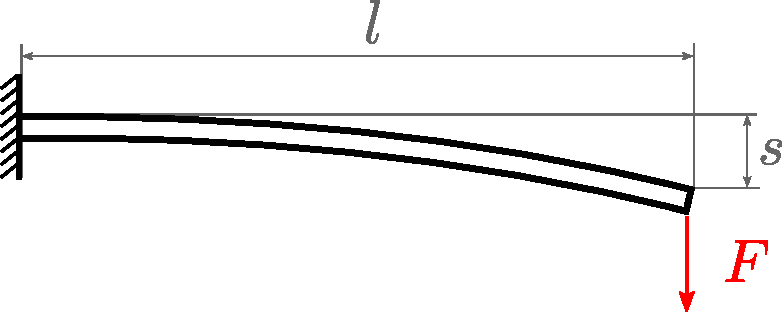
\includegraphics[width=0.5\textwidth]{figures/bending-test/setup.pdf}
\caption{Experimental setup}
\label{fig:bending-test}
\end{figure}

The elastic modulus can then be calculated depending on the cross section geometry using the equations in Table~\ref{tbl:bending-test}.

\begin{table}[H]
\centering
\begin{tabular}{| c | l |}
\hline
\textbf{Test geometry} & \textbf{Elastic Modulus} \\ \hline
\raisebox{-.5\height}{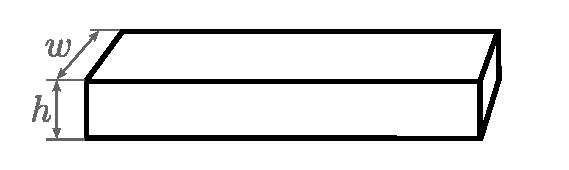
\includegraphics[width=0.4\textwidth]{figures/bending-test/sections-uniform.pdf}} & $\displaystyle E = \frac{4}{wh^3}\,\frac{Fl^3}{s}$ \\ \hline
\raisebox{-.5\height}{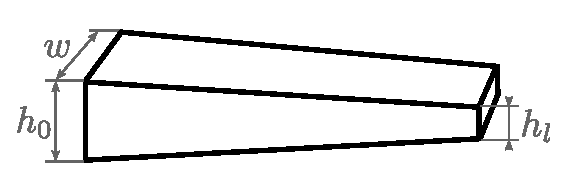
\includegraphics[width=0.4\textwidth]{figures/bending-test/sections-tapered.pdf}} & $\displaystyle E = \frac{12\,\ln(h_{l}\,l)+6}{w\,(h_{l}-h_{0})^3}\,\frac{Fl^3}{s}$ \\ \hline
\end{tabular}
\caption{Elastic modulus for different test geometries}
\label{tbl:bending-test}
\end{table}

Here are a few practical considerations:

\begin{itemize}
\item The precision of the cross sections is very important, especially the height.
\item The equations above hold for slender beams and small deflections. The test setup should be chosen accordingly. As a rule of thumb: $h, s < l/15$.
\item A simple way to apply a defined force is to hang a mass $m$ onto the beam tip and use $F = m\cdot g$, with $g = \unit[9.81]{m/s^2}$.
\item If there is some small initial deflection due to gravity, then $s$ is simply the difference in deflection after application of the force.
\end{itemize}

\end{document}